\documentclass{ctexart}
\usepackage{PhysicalChemistryNote}

\begin{document}\pagestyle{plain}
\setcounter{footnote}{0}
\begin{center}
    \tbf{\Huge Chapter 7 化学反应动力学}
\end{center}\vspace{15pt}

\indent 想象一下:你小心翼翼地把面团塞进烤箱,等待它膨胀成蓬松的面包——但如果你打开烤箱的瞬间,%
面团就“唰”地变成了焦炭,或者干脆像被施了冰冻咒一样毫无变化,厨房大概会变成灾难现场吧?%
好在现实中,大多数化学反应都像一位慢性子的老管家,不慌不忙地按照自己的节奏工作.%
而化学动力学的使命,就是破解这位管家藏在围裙口袋里的“日程表”,%
搞清楚它为何有时慢吞吞,有时又像被踩了尾巴的猫一样蹿得飞快(比如嘭一声炸开的爆米花).\\
\indent 如果说热力学是化学界的“预言家”,只告诉你“面包最终会不会烤熟”,%
那么动力学就是那个举着秒表,贴着烤箱玻璃偷看的厨师.%
它不仅关心反应的终点,更执着于追踪过程中每一个微妙的时间刻度:为什么加一撮酵母能让面团在半小时内膨胀,而不是半年?%
为什么夏天牛奶变质的速度总让冰箱成为人类最伟大的发明之一?%
这些看似平常的现象背后,都藏着分子世界速度与激情的故事.\\
\indent 准备好了吗?带上你的好奇心(和计算器),我们要推开一扇新世界的大门了——%
在这里,时间不再是钟表的滴答声,而是分子们踢踏舞步的节奏,是能量起伏的山丘地图,更是人类掌控物质变换的终极秘籍.%
祝你好运!
\newpage\documentclass{ctexart}
\usepackage{PhysicalChemistryNote}

\begin{document}\pagestyle{plain}
\noindent\tbf{\LARGE 7A 化学反应的速率与速率方程}\vspace{15pt}\\
\indent 通常,化学反应的进行总是需要一定时间.有些反应总是进行得很快(例如炸药的爆炸),%
而有些反应的速度却相当让人着急(比如无催化剂下\ce{N2}与\ce{H2}反应生成\ce{NH3}).%
于是,我们希望用一种普适的量描述化学反应的速率,并且想办法求出速率与各个反应物的浓度的关联.\vspace{12pt}\\
\Section{7A.1 化学反应的速率}
\indent 我们先从速率如何定义入手学习描述反应速率的方法.
\begin{derivation}
    朴素地来看,如果单位时间内产生的产物(或消耗的反应物)越多,那么反应的速率应当越快.%
    不过,由于物质的量$n$是广度量,因此如果用它的变化衡量速率,就会出现与系统规模有关的问题.%
    因此,我们采用一定时间内某组分浓度的变化衡量反应速率是相对合理的.\\
    于是组分$i$的反应速率$v_i$就满足
    \[v_i=\dfrac{\di[i]}{\di t}=\dfrac{1}{V}\dfrac{\di n_i}{\di t}\]
    由于反应中各物质的计量数可能并不相同,因此用上面的方法得出的速率也各有差别.%
    回忆我们在热力学中消除这一影响的方法(见\tbf{5A.1.1}),我们可以用反应进度$\xi$代替$n_i$.这样就有
    \[v_i=\dfrac{1}{V}\dfrac{\di n_i}{\di t}=\nu_i\cdot\dfrac{1}{V}\dfrac{\di\xi}{\di t}\]
    这样,我们可以得到一个统一的速率$v=\dfrac{1}{V}\dfrac{\di\xi}{\di t}$.结合计量数$\nu_i$,就可以得出任意组分的反应速率$v_i$.
\end{derivation}
\begin{definition}[7A.1.1 化学反应的速率]
    (体积不变的均相系统中的)\tbf{化学反应的速率}$r$定义为反应进度$\xi$对时间$t$的变化率与系统体积$V$的比值,即
    \[v\xlongequal{\text{def}}\dfrac{1}{V}\dfrac{\di\xi}{\di t}\]
    对于非均相系统,常常
\end{definition}
从上面的推导中很容易得出速率与各物质产生/消耗的速率的关系.
\begin{theorem}[7A.1.2 反应速率与各物质生成/消耗速率的关系]
    
\end{theorem}
\end{document}
\newpage\documentclass{ctexart}
\usepackage{PhysicalChemistryNote}

\begin{document}\pagestyle{plain}
\noindent\tbf{\LARGE 7B 积分速率方程}\vspace{15pt}\\
\indent 如我们前面所述,速率方程事实上是一个关于物质浓度的微分方程,因而可以通过数学方法求解各物质浓度与时间的关系,称为\tbf{积分速率方程}.%
在大多数情形下,这些微分方程都有精确的解析解\footnote{即有明确函数表达式的解.}.%
我们将在本节讨论常见速率方程及其解,并由此介绍其应用.\vspace{12pt}\\
\Section{7B.1 简单整数级反应的积分速率方程}
\Part{零级反应}
\indent 我们从最简单的零级反应入手.零级反应的积分速率方程的推导如下.
\begin{derivation}
    考虑零级反应\ce{A -> P},其速率方程为
    \[v=-\dfrac{\di\con{A}}{\di t}=k\]
    这是一个再简单不过的微分方程,我们移项可得
    \[\di\con{A}=-k\di t\]
    考虑起始时间为$0$,\ce{A}的起始浓度为$\con{A}_0$,对上式两边积分可得
    \[\con{A}-\con{A}_0=-kt\]
    即
    \[\con{A}=\con{A}_0-kt\]
    这表明$\con{A}$与时间$t$成一次函数关系.我们在下图中给出了\ce{A}的浓度随时间变化的图像.
    \begin{tightcenter}
        \documentclass{standalone}
\usepackage{PhysicalChemistryNote}
\begin{document}
\begin{tikzpicture}
    \draw[->] (0,0)--(6.5,0) node[right] {$t$};
    \draw[->] (0,0)--(0,4.5) node[above] {$\con{A}$};
    \draw[-] (0,4)--(6,0);
    \draw[-] (0,4)--(2,0);
    \fill (0,4) circle (1.5pt) node[left] {$\con{A}_0$};
    \fill (2,0) circle (1.5pt) node[below] {$t_1$};
    \fill (6,0) circle (1.5pt) node[below] {$t_2$};
    \node[right] at (1,2) {$k_1$};
    \node[right] at (3.1,2) {$k_2$};
\end{tikzpicture}
\end{document}
    \end{tightcenter}
    在\ce{A}反应完全后,反应便不再进行,保持$\con{A}=0$.
\end{derivation}
\begin{theorem}[7B.1.1 零级反应的积分速率方程]
    对于零级反应\ce{A -> P},其积分速率方程为
    \[\con{A}=\con{A}_0-kt\]
    其中$k$为速率常数,$\con{A}_0$为\ce{A}的起始浓度.
\end{theorem}
\Part{一级反应}
\indent 一级反应的积分速率方程的推导如下.
\begin{derivation}
    考虑一级反应\ce{A -> P},其速率方程为
    \[v=-\dfrac{\di\con{A}}{\di t}=k\con{A}\]
    同样移项可得
    \[\dfrac{\di\con{A}}{\con{A}}=-k\di t\]
    考虑起始时间为$0$,\ce{A}的起始浓度为$\con{A}_0$,对上式两边积分可得
    \[\int_{\con{A}_0}^{\con{A}}\dfrac{1}{\con{A}}\di\con{A}=-\int_0^{t}k\di t\]
    注意到$\displaystyle\int \dfrac{1}{x}\dx=\ln x$,于是上式即
    \[\ln\con{A}-\ln\con{A}_0=-kt\]
    即
    \[\ln\dfrac{\con{A}}{\con{A}_0}=-kt\ \ \ \ \ \con{A}=\con{A}_0\e^{-kt}\]
    如果将$\ln\con A$对$t$作图,将得到一条斜率为$-k$,截距为$\ln\con{A}_0$的直线.\\
    从上面的表达式可以看出,$\con{A}$的浓度随时间呈现负指数衰减.我们也在下图中给出了\ce{A}的浓度随时间变化的图像.
    \begin{tightcenter}
        \input{picture/first-order-reaction.tex}
    \end{tightcenter}
    可以看到,\ce{A}被消耗的速率随着时间而减缓.
\end{derivation}
\begin{theorem}[7B.1.2 一级反应的积分速率方程]
    对于一级反应\ce{A -> P},其积分速率方程为
    \[\con{A}=\con{A}_0\e^{-kt}\]
    其中$k$为速率常数,$\con{A}_0$为\ce{A}的起始浓度.
\end{theorem}
一级反应的速率的一个重要的指示是\tbf{半衰期}.
\begin{definition}[7B.1.3 半衰期]
    对于某个反应,某反应物浓度降低至原来的一半所用的时间为反应的\tbf{半衰期},记作$t_{1/2}$或$t_{\frac12}$.
\end{definition}
一级反应的半衰期是特殊的.
\begin{derivation}
    在\tbf{7B.1.2}的推导中有
    \[\ln\dfrac{\con{A}}{\con{A}_0}=-kt\]
    令$\dfrac{\con{A}}{\con{A}_0}=\dfrac12$,就可以得到
    \[kt_{1/2}=\ln2\]
    即$t_{1/2}=\dfrac{\ln2}{k}$.这表明一级反应的半衰期与反应物的起始浓度无关,仅与速率常数有关.
\end{derivation}
\begin{theorem}[7B.1.4 一级反应的半衰期]
    一级反应的半衰期$t_{1/2}=\dfrac{\ln 2}{k}$,是仅与速率常数有关的值.%
    因此,在相同的条件下,反应物浓度每降低一半所用的时间是定值.
\end{theorem}
我们将在后面看到,除了一级反应外,其余反应的半衰期都是与起始浓度有关的值.%
因此,有固定的半衰期这一点可以作为判断反应是否是一级的依据.\vspace{4pt}\\
\Part{二级反应}
\indent 相对而言,二级反应就比较复杂了.我们先讨论由一种反应物生成产物的二级反应.
\begin{derivation}
    考虑二级反应\ce{A -> P},其速率方程为
    \[v=-\dfrac{\di\con{A}}{\di t}=k\con{A}^2\]
    同样移项可得
    \[\dfrac{\di\con{A}}{\con{A}^2}=-k\di t\]
    考虑起始时间为$0$,\ce{A}的起始浓度为$\con{A}_0$,对上式两边积分可得
    \[\int_{\con{A}_0}^{\con{A}}\dfrac{1}{\con{A}^2}\di\con{A}=-\int_0^{t}k\di t\]
    注意到$\displaystyle\int \dfrac{1}{x^2}\dx=-\dfrac{1}{x}$,于是上式即
    \[\dfrac{1}{\con{A}_0}-\dfrac{1}{\con{A}}=-kt\]
    即
    \[\con{A}=\dfrac{\con{A}_0}{1+kt\con{A}_0}\]
    如果将$\dfrac{1}{\con{A}}$对$t$作图,将得到一条斜率为$k$,截距为$\dfrac{1}{\con{A}_0}$的直线.\\
    从上面的表达式可以看出,$\con{A}$的浓度随时间呈现倒数衰减.我们也在下图中给出了\ce{A}的浓度随时间变化的图像.
    \begin{tightcenter}
        \documentclass{standalone}
\usepackage{PhysicalChemistryNote}
\begin{document}
\begin{tikzpicture}
    \draw[->] (0,0)--(5.5,0) node[right] {$t$};
    \draw[->] (0,0)--(0,3.5) node[above] {$\dfrac{1}{\con{A}}$};
    \draw[-] (0,0.5)--(21/4,3);
    \draw[-] (0,0.5)--(1.75,3);
    \fill (0,0.5) circle (1.5pt) node[left] {$\dfrac{1}{\con{A}_0}$};
    \node[right] at (0.8,1.5) {$k_1$};
    \node[right] at (2.5,1.5) {$k_2$};
\end{tikzpicture}
\begin{tikzpicture}
    \draw[->] (0,0)--(5,0) node[right] {$t$};
    \draw[->] (0,0)--(0,3.5) node[above] {$\con{A}$};
    \draw[domain=0:5] plot[smooth](\x,{3/(1+1.5*\x)});
    \draw[domain=0:5] plot[smooth](\x,{3/(1+\x/2)});
    \fill (0,3) circle (1.5pt) node[left] {$\con{A}_0$};
    \node[right] at (0.8,1.5) {$k_1$};
    \node[right] at (2.5,1.5) {$k_2$};
\end{tikzpicture}
\end{document}
    \end{tightcenter}
    可以看到,\ce{A}被消耗的速率也随着时间而减缓,并且减缓的速度相对一级反应更大.\\
    如果令$\con{A}=\dfrac12\con{A}_0$,可得
    \[t_{1/2}=\dfrac{1}{k\con{A}_0}\]
    可见二级反应的半衰期与反应物浓度成反比例关系.
\end{derivation}
\begin{theorem}[7B.1.5 二级反应的积分速率方程I]
    对于二级反应\ce{A -> P},其积分速率方程为
    \[\dfrac{1}{\con{A}}=\dfrac{1}{\con{A}_0}+kt\ \ \text{或}\ \ \con{A}=\dfrac{\con{A}_0}{1+k\con{A}_0t}\]
    其中$k$为速率常数,$\con{A}_0$为\ce{A}的起始浓度.其半衰期为
    \[t_{1/2}=\dfrac{1}{k\con{A}}\]

\end{theorem}
现在让我们考虑更复杂的情形,即有两种反应物的二级反应.
\begin{derivation}
    考虑二级反应\ce{A + B -> P},其速率方程为
    \[v=k\con{A}\con{B}\]
    为了统一变量,不妨令$\dfrac{\xi}{V}=x$,这样根据计量数就有
    \[\con{A}=\con{A}_0-x\ \ \ \ \ \con{B}=\con{B_0}-x\]
    于是速率方程即
    \[\dfrac{\di x}{\di t}=k\left(\con{A}_0-x\right)\left(\con{B}_0-x\right)\]
    上式移项即可得
    \[\dfrac{\dx}{\left(\con{A}_0-x\right)\left(\con{B}_0-x\right)}=k\di t\]
    当$\con{A}_0=\con{B}_0$时,情形与一种反应物类似,这里不再赘述.当$\con{A}_0\neq\con{B}_0$时,%
    为了便于求积分,我们对左边的式子稍作拆分即可得
    \[\dfrac{1}{\con{B}_0-\con{A}_0}\left(\dfrac{1}{\con{A}_0-x}-\dfrac{1}{\con{B}_0-x}\right)\di x=k\di t\]
    $t=0$时$x=0$,将上式两端求定积分即可得
    \[\dfrac{1}{\con{B}_0-\con{A}_0}\left(\ln\dfrac{\con{A}}{\con{A}_0-x}-\ln\dfrac{\con{B}_0}{\con{B}_0-x}\right)=kt\]
    我们将$\con{A}=\con{A}_0-x$和$\con{B}=\con{B_0}-x$代入上式并整理,就可得
    \[\ln\dfrac{\con{B}/\con{B}_0}{\con{A}/\con{A}_0}=\left(\con{B}_0-\con{A}_0\right)kt\]
    因此,$\ln\dfrac{\con{B}}{\con{A}}$对时间$t$作图应当得到一条直线.
\end{derivation}
\begin{theorem}[7B.1.6 二级反应的积分速率方程I]
    对于二级反应\ce{A + B -> P},当$\con{A}_0\neq\con{B}_0$时,其积分速率方程为
    \[\dfrac{1}{\con{B}_0-\con{A}_0}\left(\ln\dfrac{\con{A}}{\con{A}_0-x}-\ln\dfrac{\con{B}_0}{\con{B}_0-x}\right)=kt\]
    其中$x=\dfrac{\xi}{V}$.上式亦可以写作
    \[\ln\dfrac{\con{B}/\con{B}_0}{\con{A}/\con{A}_0}=\left(\con{B}_0-\con{A}_0\right)kt
    \ \ \text{或}\ \ 
    \ln\dfrac{\con{B}}{\con{A}}=\left(\con{B}_0-\con{A}_0\right)kt+\ln\dfrac{\con{B}_0}{\con{A}_0}\]

\end{theorem}
\vspace{8pt}
\Section{7B.2 积分速率方程表}
\indent 一些简单的整数级反应的积分速率方程,我们已经在\tbf{7B.1}中介绍得比较清楚了.%
对于更为复杂的反应,不过是求解更复杂的微分方程,这需要你掌握相当高的数学功底和技巧.%
因此,我们在这里仅给出一些反应积分速率方程,其推导过程(不要求掌握)附在本节之后以供参考.
\begin{theorem}[7B.2.1 积分速率方程表]
    \begin{enumerate}[topsep=0pt,parsep=0pt,itemsep=0pt,partopsep=0pt,label=\tbf{\arabic*.}]
        \item 零级反应\ce{A -> P}
            \[v=k\ \ \ \ \ \con{A}=\con{A}_0-kt\]
        \item 一级反应\ce{A -> P}
            \[v=k\con{A}\ \ \ \ \ \con{A}=\con{A}_0\e^{-kt}\]
        \item 二级反应\ce{A -> P}
            \[v=k\con{A}^2\ \ \ \ \ \con{A}=\dfrac{\con{A}_0}{1+k\con{A}_0t}\]
        \item 二级反应\ce{A + B -> P}
            \[v=k\con{A}\con{B}\ \ \ \ \ \ln\dfrac{\con{B}/\con{B}_0}{\con{A}/\con{A}_0}=\left(\con{B}_0-\con{A}_0\right)kt\]
        \item $n$级反应\ce{A -> P}($n\geqslant2$)
            \[v=k\con{A}^n\ \ \ \ \ \dfrac{1}{n-1}\left(\dfrac{1}{\con{A}^{n-1}}-\dfrac{1}{\con{A}_0^{n-1}}\right)=kt\]
        \item 三级反应\ce{A + 2B -> P}
            \[v=k\con{A}\con{B}^2\ \ \ \ \ 
            \dfrac{2\con{P}}{\left(2\con{A}_0-\con{B}_0\right)\left(\con{B}_0-2\con{P}\right)\con{B}_0}
            +\dfrac{1}{\left(2\con{A}_0-\con{B}_0\right)^2}\ln\dfrac{\con{A}_0\left(\con{B}_0-2\con{P}\right)}
            {\left(\con{A}_0-\con{P}\right)\con{B}_0}\]
        
    \end{enumerate}
\end{theorem}
一般而言,掌握前四个就已经足够.我们现在给出\tbf{5.}和\tbf{6.}的证明.
\begin{problem}[P.7B.1]
    求$n$级反应\ce{A -> P}的积分速率方程.
\end{problem}
\begin{proof}
    我们有
    \[v=-\dfrac{\di\con{A}}{\di t}=k\con{A}^n\]
    移项可得
    \[\dfrac{\di\con{A}}{\con{A}^n}=-kt\]
    由于$\displaystyle\int\dfrac{\di x}{x^n}=-\dfrac{1}{(n-1)x^{n-1}}$,于是对上式两端求定积分可得
    \[\dfrac{1}{n-1}\left(\dfrac{1}{\con{A}^{n-1}}-\dfrac{1}{\con{A}_0^{n-1}}\right)=kt\]

\end{proof}
\begin{problem}[P.7B.1]
    求三级反应\ce{A + 2B -> P}的积分速率方程.
\end{problem}
\begin{proof}
    设$x=\dfrac{\xi}{V}$,于是
    \[v=\dfrac{\di x}{\di t}=k\con{A}\con{B}^2\]
    将$\con{A}=\con{A}_0-x,\con{B}=\con{B}_0-2x$代入可得
    \[\dfrac{\di x}{\left(\con{A}_0-x\right)\left(\con{B}_0-2x\right)^2}=k\di t\]
    若$\con{B}_0=2\con{A_0}$,那么这与单反应物的三级反应一致.否则,不妨设
    \[\dfrac{1}{\left(\con{A}_0-x\right)\left(\con{B}_0-2x\right)^2}
    =\dfrac{a}{\con{A}_0-x}+\dfrac{b}{\con{B}_0-2x}+\dfrac{c}{\left(\con{B}_0-2x\right)^2}\]
    比较系数可得
    \[a=\dfrac{1}{\left(2\con{A}_0-\con{B}_0\right)^2}\ \ \ \ \ 
    b=-\dfrac{2}{\left(2\con{A}_0-\con{B}_0\right)^2}\ \ \ \ \ 
    c=\dfrac{2}{2\con{A}_0-\con{B}_0}\]
    于是对原式两边积分可得
    \[a\ln\dfrac{\con{A}_0}{\con{A}_0-x}
    +\dfrac{b}{2}\ln\dfrac{\con{B}_0}{\con{B}_0-2x}
    +\dfrac{c}{2}\left(\dfrac{1}{\con{B}_0}-\dfrac{1}{\con{B}_0-2x}\right)=kt\]
    将$a,b,c$代入上式即可得
    \[\dfrac{1}{\left(2\con{A}_0-\con{B}_0\right)^2}
    \left(\ln\dfrac{\con{A}_0}{\con{A}_0-x}-\ln\dfrac{\con{B}_0}{\con{B}_0-2x}\right)
    +\dfrac{1}{2\con{A}_0-\con{B}_0}\left(\dfrac{1}{\con{B}_0}-\dfrac{1}{\con{B}_0-2x}\right)=kt\]
    考虑到$x=\con{P}$,于是代入并整理可得
    \[\dfrac{2\con{P}}{\left(2\con{A}_0-\con{B}_0\right)\left(\con{B}_0-2\con{P}\right)\con{B}_0}
    +\dfrac{1}{\left(2\con{A}_0-\con{B}_0\right)^2}\ln\dfrac{\con{A}_0\left(\con{B}_0-2\con{P}\right)}
    {\left(\con{A}_0-\con{P}\right)\con{B}_0}\]

\end{proof}
看到这里,你应当发现所有与此类似的整数级反应实际上不过是有理因式的积分罢了.%
这样的积分都可以通过待定系数法得出解析解.我们不希望你与这样枯燥乏味的数学做过多纠缠,%
而应当把精力放在与化学关系更大的地方,所以这一节的内容仅作为参考.
\end{document}
\newpage\documentclass{ctexart}
\usepackage{PhysicalChemistryNote}

\begin{document}\pagestyle{plain}
\noindent\tbf{\LARGE 7C 反应机理与速率方程的推导}\vspace{15pt}\\
\indent 化学反应在大多数情况下并不是一蹴而就的.例如葡萄糖\ce{C6H12O6}在你的身体里被氧化的过程:%
\ce{C6H12O6 + 6O2 -> 6CO2 + 6H2O}.显然,让一个\ce{C6H12O6}分子与六个\ce{O2}分子一步到位地生成%
六个\ce{CO2}分子与六个\ce{6H2O}分子是不大现实的,这需要所有\ce{O2}同时以合适的角度接近并发生反应,%
这一概率是非常低的.事实上我们知道,这一反应,乃至绝大多数反应都是通过数个步骤进行的,%
这些步骤构成了我们所讲的反应机理,并且也密切影响着反应的速率.\vspace{12pt}\\
\Section{7C.1 基元反应}
\Part{基元反应}
\indent 在前言中,我们说大部分反应都是通过数个步骤进行的.这些简单而基本的步骤就是我们所说的\tbf{基元反应}.
\begin{definition}[7C.1.1 基元反应]
    \tbf{基元反应}(或称\tbf{基本反应}),顾名思义,即最简单的化学反应步骤,是一个或多个化学物种直接作用,一步(即通过单一过渡态)转化为反应产物的过程.
\end{definition}
下面是几个常见的基元反应:
\begin{tightcenter}
    \ce{H. + Br2 -> HBr + Br.}\\
    \ce{CH3I + Cl- -> CH3Cl + I-}\\
    \ce{I2 -> 2I.}
\end{tightcenter}
可以看到,参与基元反应的物质并不一定是稳定的化合物,也可能是自由基等不稳定物种.并且,参与反应的分子数各不相同.
\begin{theorem}[7C.1.2 基元反应的分子数]
    基元反应的\tbf{分子数}是指参与基元反应的分子数.\\
    在\tbf{单分子反应}中,单个分子振动分解或发生重排.\\
    在\tbf{双分子反应}中,参与反应的两个分子以合适的方式碰撞,发生能量交换,键的生成和断裂等过程.\\
    一般而言,三分子反应已经很少见,而分子数大于等于四的基元反应几乎不存在.
\end{theorem}
基元反应,正由于其简单的特征,速率方程也十分简洁.
\begin{theorem}[7C.1.3 基元反应的速率方程]
    单分子基元反应对反应物为一级,其速率(以\ce{A -> P}为例)为$v=k\con{A}$.\\
    双分子基元反应对每个反应物都为一级(如果反应物相同就为二级),其速率(以\ce{A + B -> P}为例)为$v=k\con{A}\con{B}$,%
    或(以\ce{2A -> P}为例)为$v=k\con{A}^2$.
\end{theorem}
我们可以对上面的结论做定性的解释.%
在一定温度下,具有适合的能量的分子在总体中占的比例是一定的.因此,参与基元反应的物质的浓度越高,%
具有适合的能量的分子的浓度就越高,反应速率也就越快,并且对每个参与反应的分子的浓度都应当%
成正比例关系.\vspace{4pt}\\
\Part{微观可逆性原理和精细平衡原理}
\indent 直觉地来看,如果将描述物质运动的方程中的时间$t$和速度$v$替换成其负值,并不影响运动方程%
的成立.因此,运动的过程是可以通过恰好相反的方向进行的,而它们遵守相同的物理规律.这就是力学中的\tbf{时间反演对称性}%
\footnote{说得粗糙一些,这和时间倒流在某种程度上是一致的.如果你看过Christopher Nolan执导的电影《信条》,可能对这样的现象会有更为直观的认识.}.
\begin{hint}
    这一“直觉”事实上在经典力学和量子力学中都可以被证明,但由于涉及到一些复杂的物理知识,故在此并不给出.\\
    需要注意的是,由于我们在这里讨论的仅仅是单个或少数几个物体(即分子),因此尚不具有统计意义.%
    这要与热力学第二定律做区分.\\
    你可以简单地认为,力学肯定的是微观过程的可逆性,而统计物理学(以及热力学)肯定的是宏观过程的不可逆性,%
    两者讨论的范畴并不相同,因此也没有矛盾之处.
\end{hint}
以上我们从力学的角度讨论了时间反演对称性.它告诉我们,化学过程中反应的微粒服从力学方程(如基元反应中反应物微粒单次碰撞行为),%
则在正,逆反应过程中所经历的途径是相同的,逆过程要经历正过程的所有状态,就像一部电影从后往前倒过来放映,%
片中的一切动作是正常放映时动作的完全逆转;同时,在沿着反应坐标移动形成并最后解体的活化络合物的组成和结构在两个方向上是相同的,只不过动量的符号相反.%
由此,我们可以提出时间反演对称在化学动力学中的表述.
\begin{theorem}[7C.1.4 微观可逆性原理]
    如果一个正反应是基元反应,那么它的逆反应也是基元反应,且正逆反应具有相同的活化络合物(即中间体).
\end{theorem}
微观可逆性原理对假设反应厉程有明显的制约:它要求设想的反应机理中任一基元反应的逆反应不应是不可能的反应.%
如四乙基铅的气相分解反应:\ce{Pb(C2H5)4 -> Pb + 4C2H5.},逆反应是不可能发生的五分子反应,所以该反应不可能是基元反应.\\
\indent 到目前为止,我们似乎仍未考虑反应达到平衡的情形.此时,总体正反应和逆反应的速率相等,%
各物质的浓度不再随时间变化.那么具体到每个基元反应上又是何种情况呢?%
为此,人们提出了精细平衡原理.
\begin{theorem}[7C.1.5 精细平衡原理]
    平衡时,宏观体系中每一个基元反应的速率一定等于其逆反应的速率.
\end{theorem}
在化学动力学的范畴中,这也是一条可以被证明的定理.因此,这从根本上否定了平衡时存在单向不可逆循环的存在.%
每个基元反应必然存在其逆反应,且平衡时正逆反应的速率相等.%
我们将在之后看到精细平衡原理对反应机理的限制.\\
\indent 最后,需要说明的是尽管基元反应都存在逆反应,但很多基元反应的逆反应的速率非常缓慢,以至于可以忽略不计,%
因此我们近似地认为这些反应是不可逆的.这与我们在\tbf{5B.3.5}中说到的一致,即在动力学中,可逆是绝对的,不可逆是相对的.\vspace{12pt}\\
\Section{7C.2 连续反应动力学}
\Part{两步连续反应的积分速率方程}
\indent 基元反应最简单的组合方式就是连续地发生,通过几个连续的步骤完成反应.例如\ce{^{239}U}衰变为%
\ce{^{239}Pu},就是通过下面的连续$\beta$衰变进行的:
\begin{tightcenter}
    \ce{^{239}U ->T[$t_{1/2}=23.5$ min] ^{239}Np ->T[$t_{1/2}=2.35$ d] ^{239}Pu}
\end{tightcenter}
现在,我们尝试用数学方法推导最简单的连续反应——两步连续反应的积分速率方程.
\begin{derivation}
    考虑连续反应
    \begin{tightcenter}
        \ce{A ->T[$k_1$] I ->T[$k_2$] P}
    \end{tightcenter}
    对于\ce{A}而言,它的消耗是一个一级反应,满足
    \[\con{A}=\con{A}_0\e^{-k_1t}\]
    而\ce{I}满足
    \[\dfrac{\di\con{I}}{\di t}=k_1\con{A}-k_2\con{I}\]
    代入$\con{A}$的表达式即有
    \[\dfrac{\di\con{I}}{\di t}+k_2\con{I}=\con{A}_0\e^{-k_1t}\]
    这是一个一阶线性常微分方程.我们已经讲过它的解法,即常数变易法.该方程对应的齐次方程
    \[\dfrac{\di\con{I}}{\di t}+k_2\con{I}=0\]
    的通解为
    \[\con{I}=C\e^{-k_2t}\]
    令$\con{I}=C(t)\e^{-k_2t}$,代入原方程即有
    \[C'(t)\e^{-k_2t}=\con{A}_0\e^{-k_1t}\]
    于是
    \[C'(t)=\con{A}_0\e^{\left(k_2-k_1\right)t}\]
    如果$k_1\neq k_2$,那么积分可得
    \[C(t)=\dfrac{\con{A}_0}{k_2-k_1}\e^{\left(k_2-k_1\right)t}+I\]
    其中$I$为待定的积分常数.代回$\con{I}$的表达式就有
    \[\con{I}=\dfrac{\con{A}_0}{k_2-k_1}\e^{-k_1t}+I\e^{-k_2t}\]
    由于起始是并没有中间产物\ce{I}的产生,因此$t=0$时$\con{I}=0$.代入上式即可得积分常数,整理可得
    \[\con{I}=\dfrac{\con{A}_0}{k_2-k_1}\left(\e^{-k_1t}-\e^{-k_2t}\right)\]
    从而反应的速率(这里以生成\ce{P}的速率计)为
    \[v=\dfrac{\di\con{P}}{\di t}=k_2\con{I}=\dfrac{k_2\con{A}_0}{k_2-k_1}\left(\e^{-k_1t}-\e^{-k_2t}\right)\]
    由于$\con{A}+\con{I}+\con{P}=\con{A_0}$总是成立,于是
    \[\con{P}=\left(1+\dfrac{k_1\e^{-k_2t}-k_2\e^{-k_1t}}{k_2-k_1}\right)\con{A}_0\]
    这就是两步连续反应的速率方程.
\end{derivation}
\begin{theorem}[7C.2.1 两步连续反应的积分速率方程]
    连续反应\ce{A ->T[$k_1$] I ->T[$k_2$] P}的积分速率方程为
    \[\con{P}=\left(1+\dfrac{k_1\e^{-k_2t}-k_2\e^{-k_1t}}{k_2-k_1}\right)\con{A}_0\]

\end{theorem}
至于更多步的连续反应,虽然在理论上不过是多次应用常数变易法解微分方程,但其计算的复杂程度却是迅速增长的\footnote{但这似乎并不妨碍某些丧心病狂的出题人考察多步连续反应的积分速率方程.}.%
因此大多数情况下,我们也不要求连续反应的精确的积分速率方程,而是采取合理的近似以简化计算.\vspace{4pt}\\
\Part{稳态近似}
\indent 当反应机理变得更加复杂(例如存在逆反应或多步连续反应时),微分方程可能就没有显式的解,%
精确求解这样的体系也会使得计算难度大幅增加.因此我们需要想办法做一些合理的近似以简化计算.%
为此,我们先观察以下情况下两步连续反应的各物质浓度随时间变化的图像.
\begin{figure}[H]
    \centering\documentclass{standalone}
\usepackage{PhysicalChemistryNote}
\begin{document}
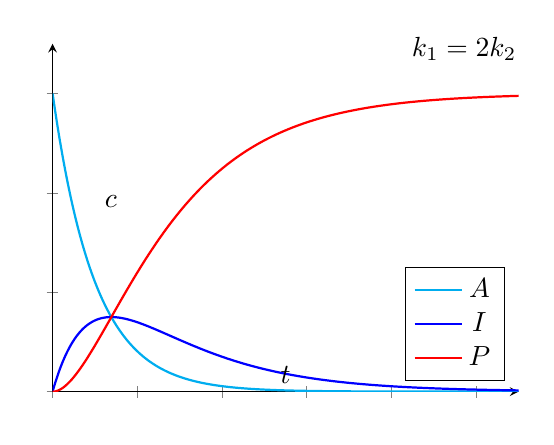
\begin{tikzpicture}
    \begin{axis}[
        title = {$k_1=2k_2$},
        title style={at={(0.75,1)},anchor=north west},
        width = 7.5cm,
        height = 6cm,
        legend pos = south east,
        x label style={at={(axis description cs:0.5,0.1)},anchor=north},
        y label style={at={(axis description cs:0.125,0.5)},rotate=270,anchor=south},
        xlabel = {$t$},
        ylabel = {$c$},
        axis lines = left,
        ymax = 3.5,
        domain = 0:5.5,
        samples = 400,
        xticklabels={},
        yticklabels={}
    ]
    \addplot [thick, cyan] {3*e^(-2*x)};
    \addplot [thick, blue] {3*(e^(-x)-e^(-2*x))};
    \addplot [thick, red] {3*(1-(2*e^(-x)-e^(-2*x)))};
    \legend {$\con{A}$,$\con{I}$,$\con{P}$}
    \end{axis}
\end{tikzpicture}
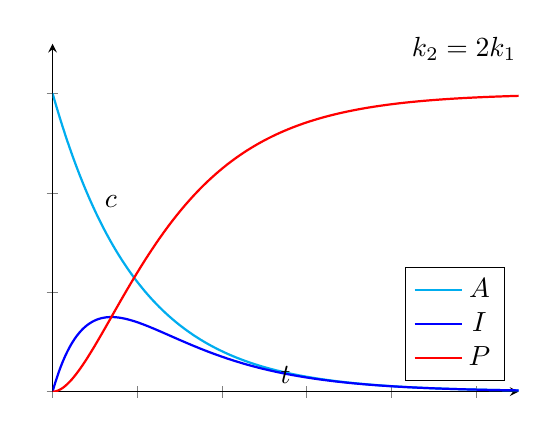
\begin{tikzpicture}
    \begin{axis}[
        title = {$k_2=2k_1$},
        title style={at={(0.75,1)},anchor=north west},
        width = 7.5cm,
        height = 6cm,
        legend pos = south east,
        x label style={at={(axis description cs:0.5,0.1)},anchor=north},
        y label style={at={(axis description cs:0.125,0.5)},rotate=270,anchor=south},
        xlabel = {$t$},
        ylabel = {$c$},
        axis lines = left,
        ymax = 3.5,
        domain = 0:5.5,
        samples = 400,
        xticklabels={},
        yticklabels={}
    ]
    \addplot [thick, cyan] {3*e^(-x)};
    \addplot [thick, blue] {3*(e^(-x)-e^(-2*x))};
    \addplot [thick, red] {3*(1-(2*e^(-x)-e^(-2*x)))};
    \legend {$\con{A}$,$\con{I}$,$\con{P}$}
    \end{axis}
\end{tikzpicture}
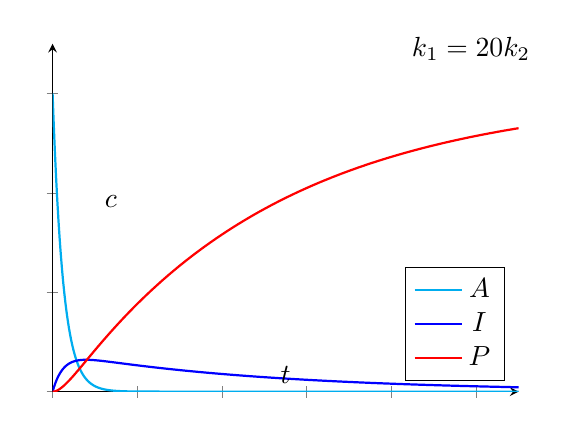
\begin{tikzpicture}
    \begin{axis}[
        title = {$k_1=20k_2$},
        title style={at={(0.75,1)},anchor=north west},
        width = 7.5cm,
        height = 6cm,
        legend pos = south east,
        x label style={at={(axis description cs:0.5,0.1)},anchor=north},
        y label style={at={(axis description cs:0.125,0.5)},rotate=270,anchor=south},
        xlabel = {$t$},
        ylabel = {$c$},
        axis lines = left,
        ymax = 3.5,
        domain = 0:5.5,
        samples = 400,
        xticklabels={},
        yticklabels={}
    ]
    \addplot [thick, cyan] {3*e^(-8*x)};
    \addplot [thick, blue] {3/7.6*(e^(-0.4*x)-e^(-8*x))};
    \addplot [thick, red] {3*(1+(0.4*e^(-8*x)-8*e^(-0.4*x))/7.6)};
    \legend {$\con{A}$,$\con{I}$,$\con{P}$}
    \end{axis}
\end{tikzpicture}
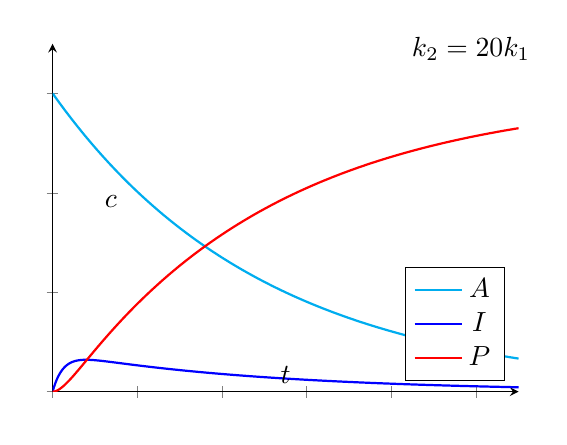
\begin{tikzpicture}
    \begin{axis}[
        title = {$k_2=20k_1$},
        title style={at={(0.75,1)},anchor=north west},
        width = 7.5cm,
        height = 6cm,
        legend pos = south east,
        x label style={at={(axis description cs:0.5,0.1)},anchor=north},
        y label style={at={(axis description cs:0.125,0.5)},rotate=270,anchor=south},
        xlabel = {$t$},
        ylabel = {$c$},
        axis lines = left,
        ymax = 3.5,
        domain = 0:5.5,
        samples = 400,
        xticklabels={},
        yticklabels={}
    ]
    \addplot [thick, cyan] {3*e^(-0.4*x)};
    \addplot [thick, blue] {3/7.6*(e^(-0.4*x)-e^(-8*x))};
    \addplot [thick, red] {3*(1+(0.4*e^(-8*x)-8*e^(-0.4*x))/7.6)};
    \legend {$\con{A}$,$\con{I}$,$\con{P}$}
    \end{axis}
\end{tikzpicture}
\end{document}
\end{figure}
当$k_1<k_2$时,
\end{document}
\newpage\documentclass{ctexart}
\usepackage{PhysicalChemistryNote}

\begin{document}\pagestyle{plain}
\noindent\tbf{\LARGE 7D 反应机理示例}\vspace{15pt}\\
\indent 在这一节中,我们将综合运用你的数学与化学知识来推导各种反应的速率方程,%
并加深你对\tbf{7C}中学习的理论知识的印象与实用的技巧.\vspace{12pt}\\
\Section{7D.1 链反应}
\Part{链反应的基本概念}
\indent 在化学动力学中有一类特殊的反应,只需用热,光或辐射等方法使反应引发,%
体系就能通过活性组分(通常是自由基或原子)相继发生一系列的连续反应,%
像链条一样自动地发展下去.
\begin{definition}[7D.1.1 链反应]
    \tbf{链反应}(又称\tbf{连锁反应}),是指反应的产物或副产物又可作为其他反应的原料,%
    从而使反应反复发生.在化学中,链反应通常在光,热,辐射或引发剂作用下,反应中交替产生活性中间体(如自由原子或自由基),%
    从而使反应一直进行下去.
\end{definition}
按照活性物质数量的变化,链反应主要有三个过程.
\begin{definition}[7D.1.2 链反应的过程]
    在链反应中,产生活性中间体的过程称为\tbf{链引发},%
    活性中间体与反应物分子反复作用生成产物的过程称为\tbf{链增长}或\tbf{链传递},%
    活性中间体最后湮灭的过程称为\tbf{链终止}.
\end{definition}
一般的链增长过程中,一个活性中间体产生一个新的活性中间体.例如\ce{Cl.}与\ce{H2}的反应:
\begin{tightcenter}
    \ce{Cl. + H2 -> HCl + H.}
\end{tightcenter}
不过,在部分链增长过程中,一个活性中间体也可能产生数个活性中间体.例如\ce{H.}与\ce{O2}的反应:
\begin{tightcenter}
    \ce{H. + O2 -> HO. + O.}
\end{tightcenter}
据此,我们可以按照链增长的性质对链反应进行分类.
\begin{definition}[7D.1.3 直链反应与支链反应]
    一个活性中间体只能产生一个新的活性中间体的反应称为\tbf{直链反应},%
    可以产生两个或多个新的活性中间体的反应称为\tbf{支链反应}.
\end{definition}
我们将在接下来对这些链反应的速率方程进行详细地讨论.\vspace{4pt}\\
\Part{直链反应——\ce{H2}与卤素单质的自由基反应}
\indent 对中间体的研究表明,\ce{H2}与\ce{X2}(其中$\ce{X}=\ce{Cl},\ce{Br},\ce{I}$)在光照或加热下的化合反应%
的机理是不同的.我们先从最简单的\ce{H2}与\ce{Cl2}的反应开始.
\begin{derivation}\setcounter{equation}{0}
    \ce{H2}与\ce{Cl2}通过自由基反应生成\ce{HCl}的反应机理如下.
    \begin{tightcenter}
        \ce{Cl2 <=>T[$k_1$][$k_{-1}$] 2Cl.}\\
        \ce{Cl. + H2 ->T[$k_2$] HCl + H.}\\
        \ce{H. + Cl2 ->T[$k_3$] HCl + Cl.}
    \end{tightcenter}
    由于产物\ce{HCl}十分稳定,因此忽略后两个反应的逆反应.\\
    体系中的不稳定中间体为\ce{H.}与\ce{Cl.},分别对它们稳态近似有
    \begin{equation}
        \dfrac{\di\con{H.}}{\di t}=k_2\con{Cl.}\con{H2}-k_3\con{H.}\con{Cl2}=0
    \end{equation}
    \begin{equation}
        \dfrac{\di\con{Cl.}}{\di t}=2k_1\con{Cl2}-2k_{-1}\con{Cl.}^2-k_2\con{Cl.}\con{H2}+k_3\con{H.}\con{Cl2}=0
    \end{equation}
    将(2)减去(1)可得
    \begin{equation}
        2k_1\con{Cl2}-2k_{-1}\con{Cl.}^2=0
    \end{equation}
    于是
    \begin{equation}
        \con{Cl.}=\sqrt{\dfrac{k_1}{k_{-1}}\con{Cl2}}
    \end{equation}
    由(1)可得
    \begin{equation}
        \dfrac{\di\con{HCl}}{\di t}=k_2\con{Cl.}\con{H2}+k_3\con{H.}\con{Cl2}=2k_2\con{Cl.}\con{H2}
    \end{equation}
    将(4)代入(5)可得
    \begin{equation}
        \dfrac{\di\con{HCl}}{\di t}=2k_2\con{Cl.}\con{H2}=2k_2\sqrt{\dfrac{k_1}{k_{-1}}}\con{H2}\con{Cl2}^{\frac12}
    \end{equation}
    因此反应对\ce{H2}为一级,对\ce{Cl2}为二分之一级.
\end{derivation}

\end{document}
\newpage\documentclass{ctexart}
\usepackage{PhysicalChemistryNote}

\begin{document}\pagestyle{plain}
\noindent\tbf{\LARGE 7E 温度对反应速率的影响}\vspace{15pt}\\
\indent 实验表明,大多数化学反应的速率总是随着温度升高而增加.我们将从理论上对此给出解释,%
并说明速率常数与温度满足的关系.在本节的最后,我们也将介绍一种测定速率常数的重要办法.\vspace{12pt}\\
\Section{7E.1 Arrhenius方程}
\indent Arrhenius研究了许多气相反应的速率,由此揭示了反应的速率常数与温度的关系.
\begin{theorem}[7E.1.1 Arrhenius方程]
    反应速率常数$k$与温度$T$满足
    \[k=A\exp\left(-\dfrac{E_a}{RT}\right)\]
    其中$A$为\tbf{指前因子},$E_a$为\tbf{表观活化能}.
\end{theorem}
尽管Arrhennius得出的$A$和$E_a$是完全经验性的,但他还是对此做出了一些合理的解释.%
他认为,并不是反应分子的每次接触都能发生反应,只有那些能量足够高的分子之间的角度合适的碰撞才能发生反应.%
这些分子被称为\tbf{活化分子},而由非活化分子变为活化分子所需要的平均能量即为\tbf{(表观)活化能}.%
由上面的定性解释,以及我们在\tbf{1B}中提到的能量分布公式,我们可以简单地推导Arrhenius方程.
\begin{derivation}
    假定能量不低于$E_{\min}$的分子才能发生反应.根据\tbf{1B.3.3},这样的分子占总体的比例为
    \[p=\exp\left(-\dfrac{E_{\min}}{k_\text{B}T}\right)\]
    令$E_a=\NA E_{\min}$.如果活化能$E_a=0$,那么每一次碰撞都会发生反应.%
    不妨记此时$k=A$,这样指前因子$A$就代表每次碰撞都发生反应时对应的速率常数.%
    当$E_a>0$时,能发生反应的分子数的比例变为$p$,那么就有
    \[k=Ap=A\exp\left(-\dfrac{E_a}{RT}\right)\]
    这个推导过程相当粗糙,因而(几乎)只起到定性的作用.
\end{derivation}
对Arrhenius方程取对数后可得
\[\ln k=\ln A-\dfrac{E_a}{RT}\]
如果$A$与$T$无关,就可以通过$\ln k$对$\dfrac1T$作图的方式确定$A$与$E_a$.我们将上式对$T$微分可得
\[\left(\dfrac{\di\ln k}{\di T}\right)=\dfrac{E_a}{RT^2}\]
这可以作为活化能的正式定义.
\begin{definition}[7E.1.2 表观活化能]
    表观活化能$E_a$可以定义为
    \[E_a=RT^2\left(\dfrac{\di\ln k}{\di T}\right)\]

\end{definition}
对于$E_a$不随$T$变化的情形,这就与前面给出的直线等价.%
而$E_a$随$T$变化则可能暗示着反应机理的改变.\\
\indent 对于复杂反应而言,总的表观活化能可以根据反应的速率方程和各基元反应的表观活化能得出.%
例如我们在前面提到的\ce{H2}与\ce{Cl2}的反应,其速率方程为
\[v=\dfrac{1}{2}\dfrac{\di\con{HCl}}{\di t}=k_2\sqrt{\dfrac{k_1}{k_{-1}}}\con{H2}\con{Cl2}^{\frac12}\]
因此表观速率常数$k_{\text{obs}}=k_2\sqrt{\dfrac{k_1}{k_{-1}}}$.于是
\[E_{a,\text{obs}}=A_2\sqrt{\dfrac{A_1}{A_{-1}}}\left(E_{a,2}+\dfrac12E_{a,1}-\dfrac12E_{a,-1}\right)\]
需要注意的是,两个自由基反应形成分子的活化能几乎为$0$,因为自由基本来就是活泼的,只要相遇几乎都能发生反应,%
因此$E_{a,-1}\approx0$.这样,上式也可以改写为
\[E_{a,\text{obs}}=A_2\sqrt{\dfrac{A_1}{A_{-1}}}\left(E_{a,2}+\dfrac12E_{a,1}\right)\]
\begin{theorem}[7E.1.3 自由基偶联反应的表观活化能]
    两个自由基偶联的反应的表观活化能$E_a$近似为$0$.
\end{theorem}
\vspace{8pt}
\Section{7E.2 过渡态理论}
\indent 虽然Arrhenius方程的确能够描述温度对反应的影响,可它毕竟是定性的,%
并没有很好地在微观层面解释反应的机制,也没有合适的理论证明其成立性.%
为了填补这一空白,Eyring等人提出了\tbf{过渡态理论},揭示了反应发生的具体过程.\vspace{4pt}\\
\Part{势能面,反应坐标与过渡态}
\indent 我们设想发生反应的是\ce{A}与\ce{B}两个分子.它们的原子分别为$\ce{A}_1,\cdots,\ce{A}_j$和$\ce{B}_1,\cdots,\ce{B}_k$.%
显然,这两个分子构成的系统的能量会随着\ce{A}与\ce{B}的相对发生变化.我们不妨用函数表示体系的能量,即
\[E=f\left(\li{\ce{A}},j,\li{\ce{B}},k\right)\]
这一函数接受所有$j+k$个原子的位置为自变量,并给出总能量\footnote{这里指势能.}$E$.%
在实际应用中,通常也会使用各个原子之间的距离$d$,键角$\theta$等参数描述原子的相对位置,%
并作为$E$的自变量.我们把系统处于某一状态下的位置信息统一为一个元素$S$,这样就有$E=f(S)$.%
所有可能的$S$组成了一个集合$X$,$X$内的任意元素都代表了各个原子的一种位置状态.
\begin{definition}[7E.2.1 势能面]
    \tbf{势能面}即表示某一微观体系的势能和相关参数(通常为原子坐标)之间的函数关系,是势能函数$E=f(S)$的图像.
\end{definition}
\indent 如果$S$是一维的,这意味着我们可以在二维平面上画出$E-S$图(正如一般的一元函数一样,这是一条曲线).%
类似地,如果$S$是二维的,就可以在三维空间中画出$E-S$的图像,这则是一片曲面.当$S$的维度更高时,%
直观上并没有$E-S$图的很好的几何对应,但其数学意义仍然是清晰的.\\
\indent 如果\ce{A}与\ce{B}发生了反应生成产物\ce{P},那么上面的集合$X$中也应当有元素$S_{\ce{P}}$,以对应所有原子组成\ce{P}的状态.%
$S_{\ce{P}}$可以从\ce{P}的结构直接得到.我们再考虑\ce{A}和\ce{B}距离足够远的状态$S_{\ce{A}+\ce{B}}$作为反应的起始状态.\\
\indent 现在,我们只需要考虑系统如何由状态$S_{\ce{A}+\ce{B}}$变为$S_{\ce{P}}$即可.%
你可以认为\ce{A}和\ce{B}都分解为独立的原子之后再组合成\ce{P},不过那样的方式太过粗暴,%
并且显然会消耗不少的能量.\ce{A}和\ce{B}会明智地选择一种能量最低的方式变成\ce{P}%
\footnote{如果我们从能量分布的角度考虑此事,就会发现能量更高的途径对应的概率更低,因此过于高能的中间状态事实上出现的概率非常小,因此不纳入考虑中.%
而系统发生变化的途径最有可能的途径正是能量最低的途径.},%
即反应发生的真实途径.我们把这一途径称为\tbf{反应坐标}.
\begin{definition}[7E.2.2 反应坐标]
    \tbf{反应坐标}(reaction coordinate)是由反应物变为产物的过程中系统状态的集合,%
    也对应势能面上连接反应物和产物的最低能量路径.
\end{definition}
反应坐标准确地描述了反应进行的过程.例如,对于\ce{A + B -> P}这一反应,系统能量与反应坐标可能具有下面的关系.
\begin{figure}[H]
    \centering\documentclass{standalone}
\usepackage{PhysicalChemistryNote}
\begin{document}
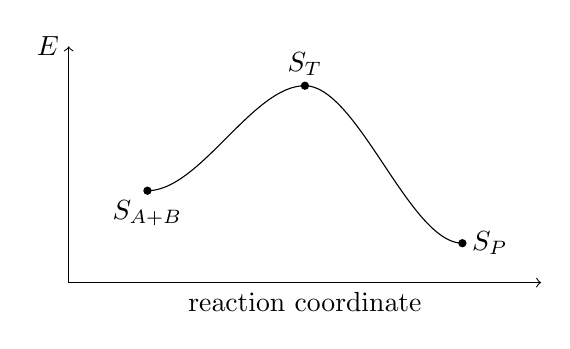
\begin{tikzpicture}
    \draw[->] (0,0)--(6,0) ;
    \node[below] at (3,0) {reaction coordinate};
    \draw[->] (0,0)--(0,3) node[left]{$E$};
    \draw[domain=1:3] plot[smooth] (\x,{(-(\x-2)^3+3*\x-0.5)/3});
    \draw[domain=3:5] plot[smooth] (\x,{((\x-4)^3-3*\x+15)/2});
    \fill (1,7/6) circle (1.5pt) node[below]{$S_{\ce{A}+\ce{B}}$};
    \fill (3,2.5) circle (1.5pt) node[above]{$S_{\ce{T}}$};
    \fill (5,0.5) circle (1.5pt) node[right]{$S_{\ce{P}}$};
    
\end{tikzpicture}
\end{document}
\end{figure}
这正是我们限制$S$在反应坐标内后得到的势能面的截面.%
并且,这条曲线的最高点对应的状态$S_{\ce{T}}$具有如下的性质.
\begin{definition}[7E.2.3 过渡态]
    \tbf{过渡态}是反应坐标中能量的最高点对应的系统状态.%
\end{definition}
\begin{theorem}[7E.2.4 过渡态的数学意义]
    过渡态是整个势能面的\tbf{鞍点}.在这一点,只有沿着反应坐标的方向变化,势能才会降低,%
    除此之外的任意方向都会使得势能升高.
\end{theorem}
下图中的中心点就是鞍点的示意.如果我们要从前面这一侧翻越到后面这一侧,那么能量最低的选择就是通过鞍点.
\begin{tightcenter}
    \documentclass{standalone}
\usepackage{PhysicalChemistryNote}
\begin{document}
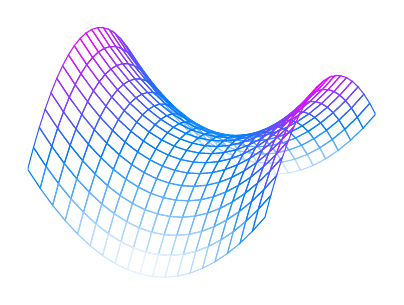
\begin{tikzpicture}
    \begin{axis}[
        hide axis,
        width=6cm,
        height=6cm,
        colormap/cool
    ]
    \addplot3[
        mesh,
        samples=20,
        domain=-1:1,
    ]
    {x^2-y^2};
    \end{axis}
\end{tikzpicture}
\end{document}
\end{tightcenter}
想象一下,你打算翻过一座山.这座山恰好有一个山坳,因此你就决定从那里过去,%
而不会傻乎乎地先爬到山顶再下山.这个山坳就是上图中的鞍点.
\begin{hint}
    作为补充,在数学上,我们通过计算Hessian矩阵判断鞍点,在鞍点处的Hessian矩阵仅有一个负本征值,对应反应坐标方向.这也是计算化学中寻找过渡态的重要依据.
\end{hint}

\indent 过渡态的物理意义在于它描述了反应物到产物的中间状态,即旧键将断未断,新键将成未成的状态.%
这一状态也被称作\tbf{活化络合物}.这需要与中间体区分.\vspace{4pt}\\
\Part{过渡态理论与Eyring方程}
\indent 我们已经找到了一种十分优秀的描述反应过程的方式,而我们并不打算止步于此.%
在做出过渡态理论的基本假设后,我们可以给出活化能的更明确的定义,并据此得出过渡态理论中的一个重要公式.
\begin{theorem}[7E.2.5 过渡态理论的基本假设]
    \begin{enumerate}[topsep=0pt,parsep=0pt,itemsep=0pt,partopsep=0pt,label=\tbf{\arabic*.},leftmargin=*]
        \item 反应物变为产物的过程总是经过势能面上的鞍点,即过渡态.
        \item 反应物和过渡态(活化络合物)总是处于准平衡态.
        \item 过渡态向产物的转化是不可逆的.
        \item \tbf{2.}和\tbf{3.}的反应也满足质量作用定律.
    \end{enumerate}
\end{theorem}
我们也可以将后两点假设表示为下面的过程.
\begin{tightcenter}
    \ce{A + B <=> T$^\ddagger$ -> P}
\end{tightcenter}
现在我们来推导描述反应速率常数的方程.
\begin{derivation}\setcounter{equation}{0}
    考虑实际反应
    \begin{tightcenter}
        \ce{A + B ->T[$k$] P}
    \end{tightcenter}
    以及过渡态\ce{T$^\ddagger$}向产物\ce{P}的转化反应
    \begin{tightcenter}
        \ce{T$^\ddagger$ ->T[$k^\ddagger$] P}
    \end{tightcenter}
    根据基本的动力学假设,我们可以得到
    \begin{equation}
        \dfrac{\di\con{P}}{\di t}=k\con{A}\con{B}=k^\ddagger\con{T^\ddagger}
    \end{equation}
    于是第一步平衡的平衡常数
    \begin{equation}
        K=\dfrac{\con{T^\ddagger}}{\con{A}\con{B}}=\dfrac{k}{k^\ddagger}
    \end{equation}
    活化络合物转化为产物的速率常数与活化络合物中的振动有关,这一振动使得活化络合物更类似于产物,从而使得活化络合物沿着反应坐标向产物方向倾斜.%
    我们把振动频率记为$\nu$.\\
    然而,不是所有振动都可以使得过渡态向产物的方向转化.分子中的其他原子可能并不能够适当地排列以使过渡态转化为产物,%
    或者分子的旋转状态妨碍了过渡态向产物的转变.只有一部分的振动可以使得我们希望的转化发生,因此我们定义\tbf{传递系数}$\kappa$表示这样的振动的所占的比例.于是就有
    \begin{equation}
        k^\ddagger=\kappa\nu
    \end{equation}
    现在我们来考虑$K$.虽然过渡态并不满足统计力学(它的留存时间太短),但我们可以采取统计力学方法%
    证明它与一个真正的平衡常数$K^\ddagger$成比例关系,即
    \begin{equation}
        K=\left(\dfrac{k_{\text B}T}{h\nu}\right)K^\ddagger
    \end{equation}
    由(2)(4)和(5)可得
    \begin{equation}
        k=Kk^\ddagger=\kappa\left(\dfrac{k_{\text B}T}{h}\right)K^\ddagger
    \end{equation}
    而由$K^\dagger$可以定义活化Gibbs自由能,活化焓和活化熵,即
    \begin{equation}
        \Delta G^\ddagger=-RT\ln K^\ddagger
    \end{equation}
    \begin{equation}
        \Delta G^\ddagger=\Delta H^\ddagger-T\Delta S^\ddagger
    \end{equation}

\end{derivation}
这样,我们就得到了Eyring方程.
\begin{theorem}[7E.2.6 Eyring方程]
    基元反应的速率常数$k$满足
    \[k=\kappa\left(\dfrac{k_\text BT}{h}\right)\exp\left(-\dfrac{\Delta G^\ddagger}{RT}\right)\]
    其中$\kappa$为\tbf{传递系数},$\Delta G^\ddagger$为活化Gibbs自由能.
\end{theorem}
我们可以改写Eyring方程得到
\[k=\left[\kappa\left(\dfrac{k_\text BT}{h}\right)\exp\left(\dfrac{\Delta S^\ddagger}{R}\right)\right]\exp\left(-\dfrac{\Delta H^\ddagger}{RT}\right)\]
如果假定$\Delta H^\ddagger$不随温度变化,那么对于基元反应,这就是Arrhenius方程的形式,其中
\[A=\kappa\left(\dfrac{k_\text BT}{h}\right)\exp\left(\dfrac{\Delta S^\ddagger}{R}\right)\ \ \ \ \ E_a=\Delta H^\ddagger\]
因此,可以认为指前因子$A$主要由活化熵$\Delta S^\ddagger$决定,而活化能$E_a$主要由活化焓$\Delta H^\ddagger$决定.\\
\indent 过渡态理论比起传统的碰撞理论是对反应过程描述的一大进步.%
它通过活化络合物模型,成功将分子动力学与宏观反应速率结合,并且为计算化学提供了%
计算反应速率的理论基础.
\begin{hint}
    如果你感到上面的内容模糊不清,并且想详细了解过渡态理论的相关内容,那么笔者建议你阅读《现代物理有机化学》一书的第七章.%
    顺带一提,这本书的所有内容都非常值得你仔细学习.
\end{hint}
\vspace{8pt}
\Section{7E.3 弛豫法测定速率常数}
\indent 我们在本章的前几节介绍了几种测定速率的简单方法.%
自然,有更加精密和先进的手段测定反应速率,不过我们并不打算介绍那些复杂的仪器与方法,%
而是介绍一种重要的,与速率方程密切相关的测定对峙反应速率常数的方法——\tbf{弛豫法}.
\begin{definition}[7E.3.1 弛豫]
    \tbf{弛豫}是指的是在某一个渐变过程中从某一个状态逐渐地恢复到平衡态的过程.
\end{definition}
对于一个处于平衡的化学反应而言,如果改变温度(这通常通过放电,激光等方式进行),那么平衡将发生移动.%
测定各种物质的浓度随时间的变化,就能获知反应的速率常数.%
我们从最简单的反应\ce{A <=> P}开始.
\begin{derivation}
    系统初始处于平衡态.我们假定改变条件后有
    \begin{tightcenter}
        \ce{A <=>T[$k_1$][$k_{-1}$] P}
    \end{tightcenter}
    并且最终平衡时\ce{A}和\ce{P}的浓度分别为$\con{A}_{\text{eq}}$和$\con{P}_{\text{eq}}$.这样就有
    \[k_1\con{A}_{\text{eq}}=k_{-1}\con{P}_{\text{eq}}\]
    令$x=\con{A}-\con{A}_{\text{eq}}=\con{P}_{\text{eq}}-\con{P}$表示反应偏离平衡的程度,就有
    \[\begin{aligned}
        \dfrac{\di\con{A}}{\di t}
        &= k_{-1}\con{P}-k_1\con{A} \\
        &= k_{-1}\left(\con{P}_{\text{eq}}-x\right)-k_1\left(\con{A}_{\text{eq}}+x\right) \\
        &= -\left(k_{-1}+k_1\right)x+k_{-1}\con{P}_{\text{eq}}-k_1\con{A}_{\text{eq}} \\
        &= -\left(k_1+k_{-1}\right)x
    \end{aligned}\]
    又因为$\dfrac{\di\con{A}}{\di t}=\dfrac{\di x}{\di t}$,于是有
    \[\dfrac{\di x}{\di t}=-\left(k_1+k_{-1}\right)x\]
    这是一个一阶微分方程,其解为
    \[x=x_0\e^{-\left(k_1+k_{-1}\right)t}\]
    其中$x_0$即为初始状态的$x$(亦即条件改变前后平衡状态时$\con{A}$或$\con{P}$之差).我们令弛豫时间$\tau=\dfrac{1}{k_1+k_{-1}}$,就有
    \[x=x_0\e^{-\frac{t}{\tau}}\]
    测定$x$依时间的变化关系,得出弛豫时间$\tau$,再结合平衡常数$K=\dfrac{k_1}{k_{-1}}$就可以得出$k_1$与$k_{-1}$.%
    这为我们测定对峙反应的正逆反应速率常数提供了一个相当不错的办法.
\end{derivation}
对于更复杂的体系,处理方法是类似的.我们以\ce{A + B <=> C + D}为例.
\begin{derivation}
    系统初始处于平衡态.我们假定改变条件后有
    \begin{tightcenter}
        \ce{A + B <=>T[$k_1$][$k_{-1}$] C + D}
    \end{tightcenter}
    同样地,平衡时有
    \[k_1\con{A}_{\text{eq}}\con{B}_{\text{eq}}=k_{-1}\con{C}_{\text{eq}}\con{D}_{\text{eq}}\]
    仍令$x=\con{A}-\con{A}_{\text{eq}}$为反应偏离平衡的程度,于是有
    \[\begin{aligned}
        \dfrac{\di x}{\di t}
        = &\ \dfrac{\di\con{A}}{\di t} = k_{-1}\con{C}\con{D}-k_1\con{A}\con{B} \\
        = &\ k_{-1}\left(\con{C}_{\text{eq}}-x\right)\left(\con{D}_{\text{eq}}-x\right)-k_1\left(\con{A}_{\text{eq}}+x\right)\left(\con{B}_{\text{eq}}+x\right) \\
        = &\ k_{-1}\con{C}_{\text{eq}}\con{D}_{\text{eq}}-k_1\con{A}_{\text{eq}}\con{B}_{\text{eq}} \\
          &\ -\left[k_{-1}\left(\con{C}_{\text{eq}}+\con{D}_{\text{eq}}\right)+k_1\left(\con{A}_{\text{eq}}+\con{B}_{\text{eq}}\right)\right]x \\
          &\ +\left(k_{-1}-k_1\right)x^2
    \end{aligned}\]
    由于我们的条件改变总是很微小的(否则也无法保证条件的改变在一瞬间内完成),因此$x$相对各物质的平衡浓度也是很小的.于是,我们忽略上式的二次项即可得
    \[\dfrac{\di x}{\di t}=-\left[k_{-1}\left(\con{C}_{\text{eq}}+\con{D}_{\text{eq}}\right)+k_1\left(\con{A}_{\text{eq}}+\con{B}_{\text{eq}}\right)\right]x\]
    这也是一个一阶微分方程.对应的弛豫时间为
    \[\tau=\dfrac{1}{k_1\left(\con{A}_{\text{eq}}+\con{B}_{\text{eq}}\right)+k_{-1}\left(\con{C}_{\text{eq}}+\con{D}_{\text{eq}}\right)}\]

\end{derivation}
\begin{theorem}[7E.3.2 弛豫法测定速率常数]
    当反应处于平衡时,给系统一个微小的扰动(例如升高温度),测定体系中物质的浓度偏离新的平衡状态的差值$x$随时间$t$的变化,%
    就可以根据前面的推导过程求出正逆反应的速率常数.
\end{theorem}
\end{document}
\newpage\documentclass{ctexart}
\usepackage{PhysicalChemistryNote}

\begin{document}\pagestyle{plain}
\noindent\tbf{\LARGE Ex7 习题}\vspace{15pt}\\
\indent 我们将在本章的习题中给出更多的例题以供你巩固动力学知识.
\setcounter{Pcounter}{0}
\stepcounter{Pcounter}
\begin{problem}[P.7.\arabic{Pcounter}]
    Heck偶联反应为代表的过渡金属催化的偶联反应.这一反应的通式如下.
    \begin{tightcenter}
        \ce{ArBr + RCH=CH2 ->T[Pd catalyst][AcONa] ArCH=CHR + AcOH + NaBr}
    \end{tightcenter}
    这一反应的机理可以简化如下.
    \begin{tightcenter}
        \ce{E + A <=>T[$k_1$][$k_{-1}$] EA} \\
        \ce{EA + B ->T[$k_2$] E + P}
    \end{tightcenter}
    其中\ce{E}为\ce{Pd}催化剂,\ce{A}为溴代物,\ce{B}为原料烯烃,\ce{P}为产物烯烃.
    \begin{enumerate}[label=\tbf{\arabic{Pcounter}-\arabic*},topsep=0pt,parsep=0pt,itemsep=0pt,partopsep=0pt]
        \item 推导总反应速率$r$(以生成产物\ce{P}的速率记)的表达式.
        \item 记$\con{ex}=\con{B}_0-\con{A}_0$为两种底物的起始浓度之差,$\con{E}_0$为催化剂的总浓度.
        \item 将$1.0\mol$ \ce{C2H5OH(g)},$3.0\mol$ \ce{C2H4(g)}和$1.0\mol$ \ce{H2O}混合,形成总压力$p=p^\ominus$的理想气体混合物.%
            通过计算判断该反应在$500\K$时进行的方向.
    \end{enumerate}
\end{problem}
\begin{solution}
    在开始求解之前,我们需要说明一点:求火焰能达到的最高温度等价于求恒压绝热反应体系能达到的最高温度.%
    因为物质燃烧是迅速的,完成反应后其热量来不及与外界交换,因而体系可以近似地看作绝热的.如果是在密闭容器内进行的爆炸过程,应当采取定容热容和反应的内能变进行计算.\\
    现在我们来考虑该体系.不妨假定发生反应之前$n(\ce{CH4})=1\mol$(这里系统的规模与火焰温度无关,因此我们可以任意地指定一个值以方便计算),发生反应
    \[\ce{CH4 + 2O2 -> CO2 + 2H2O}\]
    因此反应前$n(\ce{O2})=2\mol,n(\ce{N2})=8\mol$.先假定系统在恒温下反应,该过程的焓变
    \[\begin{aligned}
        \Delta_\r H_1
        &= \sum_i n_i\Delta_\f H_{\m,i}^\ominus \\
        &= 1\cdot\left((-393.51)+2\times(-241.82)-(-74.6)+0\right)\kJm \\
        &= -802.55\kJm
    \end{aligned}\]
    反应后,系统的组成为$1\mol$ \ce{CO2},$2\mol$ \ce{H2O},$8\mol$ \ce{N2}.系统的定压热容为
    \[\begin{aligned}
        C_{p,\text{tot}}
        &= \sum_in_iC_{p,\m,i} \\
        &= \left[(44.22+2\times30.00+8\times28.58)+(8.79+2\times10.7+8\times3.77)\times10^{-3}\right]\text{J}\cdot\text K^{-1} \\
        &= \left(332.86+60.35\times10^{-3}T\right)\text{J}\cdot\text K^{-1}
    \end{aligned}\]
    假定最终系统的温度为$T_1\K$,那么升温过程的焓变
    \[\begin{aligned}
        \Delta H_2
        &= \int_{298.15\K}^{T_1\K}C_{p,\text{tot}}\di T \\
        &= \int_{298.15\K}^{T_1\K}\left(332.86+60.35\times10^{-3}T\right)\di T \\
        &= \left(-101924.57+332.86T_1+30.18T_1^2\right)\text J
    \end{aligned}\]
    由于该过程是等压绝热过程,因此$\Delta H_{\text{tot}}=Q_p=0$,于是$\Delta_\r H_1+\Delta H_2=0$.于是
    \[\left(-101924.57+332.86T_1+30.18T_1^2\right)\text J=-802.55\text{ kJ}\]
    解得$T_1=2256$.于是火焰温度最高为$2256\K$.
\end{solution}

\end{document}
\end{document}